\section{Experiments}


In this section, we conduct extensive experiments to address the following research questions (RQs): \textbf{RQ1:} How can user strategies influence the ecosystem evolution based on individual rationality? \textbf{RQ2:} How does the validation mechanism affect the net welfare within the ecosystem?  \textbf{RQ3:} What is the relationship between the service quality and overall welfare?





% \begin{figure*}[t]
%     \centering

%     \caption{roc.}
    
%     \label{fig:five-images}
% \end{figure*}


% \begin{figure*}[t]
%     \centering
%     \begin{subfigure}[b]{0.162\linewidth}
%         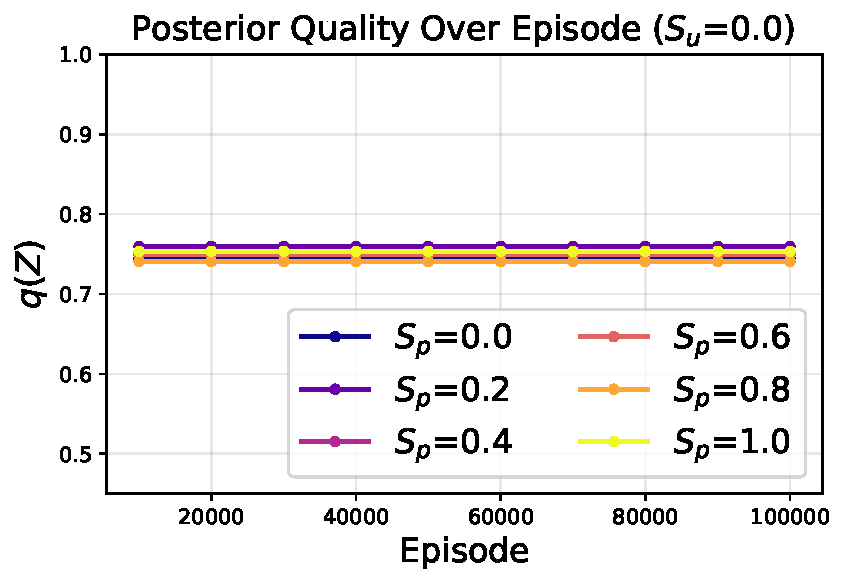
\includegraphics[width=\linewidth]{figures/fixed_su/user_strategy_0_0_weighted_p.png}
%         \caption{0}
%     \end{subfigure}
%     % \hfill
%     \begin{subfigure}[b]{0.162\linewidth}
%         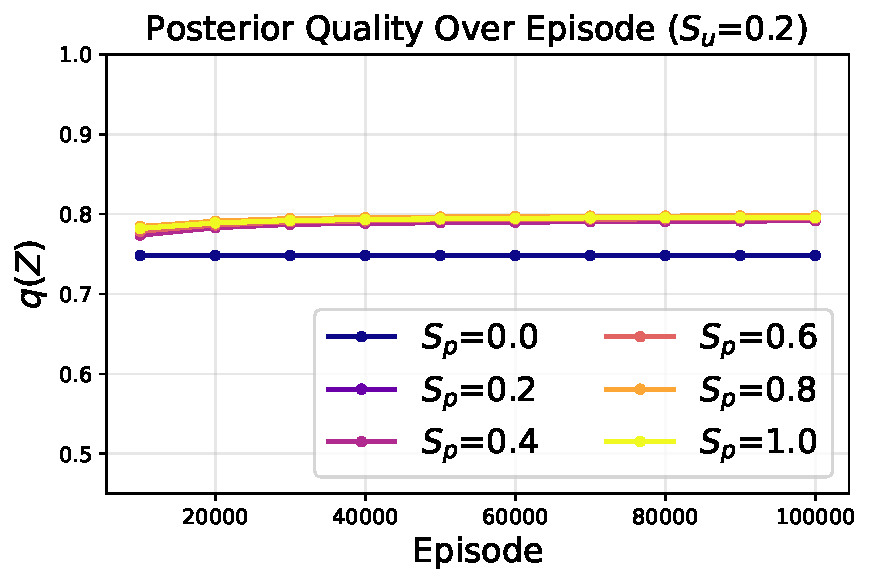
\includegraphics[width=\linewidth]{figures/fixed_su/user_strategy_0_2_weighted_p.png}
%         \caption{0.2}
%     \end{subfigure}
%     % \hfill
%     \begin{subfigure}[b]{0.162\linewidth}
%         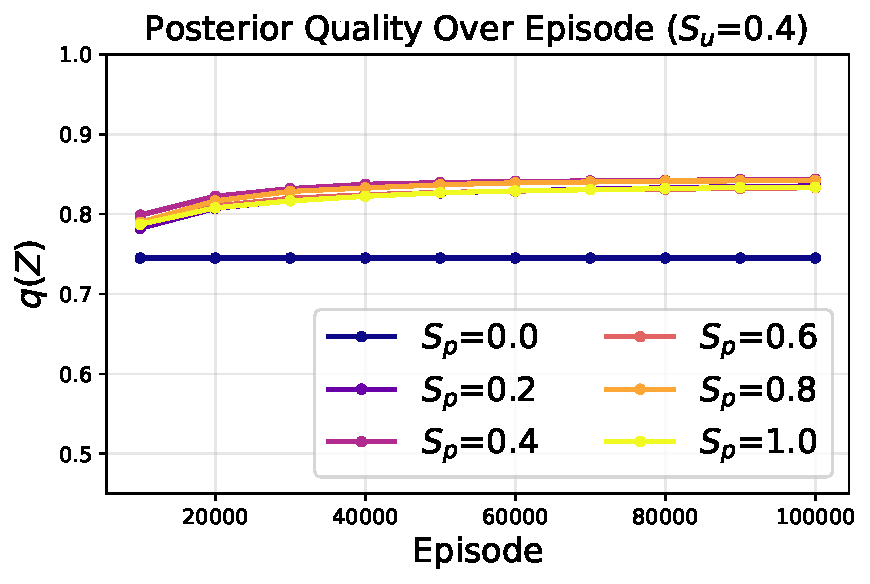
\includegraphics[width=\linewidth]{figures/fixed_su/user_strategy_0_4_weighted_p.png}
%         \caption{0.4}
%     \end{subfigure}
%     % \hfill
%     \begin{subfigure}[b]{0.162\linewidth}
%         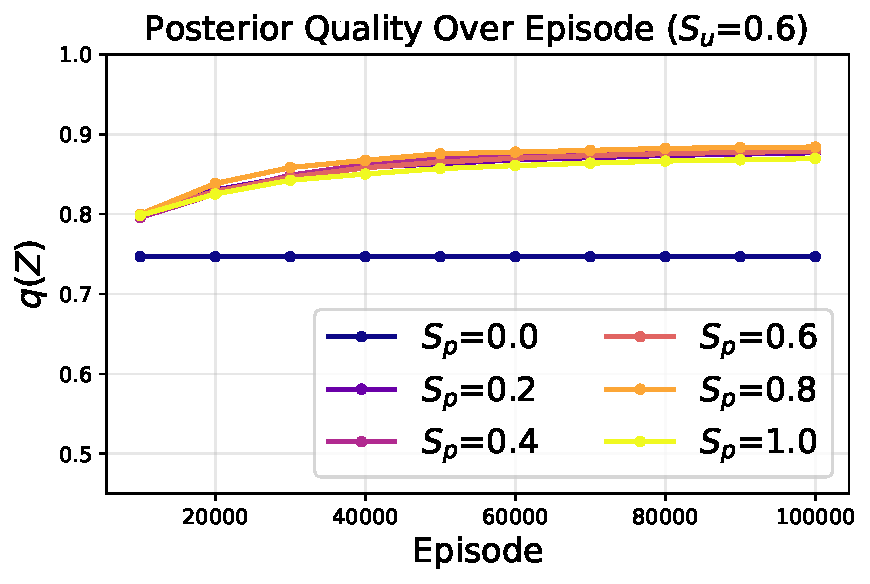
\includegraphics[width=\linewidth]{figures/fixed_su/user_strategy_0_6_weighted_p.png}
%         \caption{0.6}
%     \end{subfigure}
%     % \hfill
%     \begin{subfigure}[b]{0.162\linewidth}
%         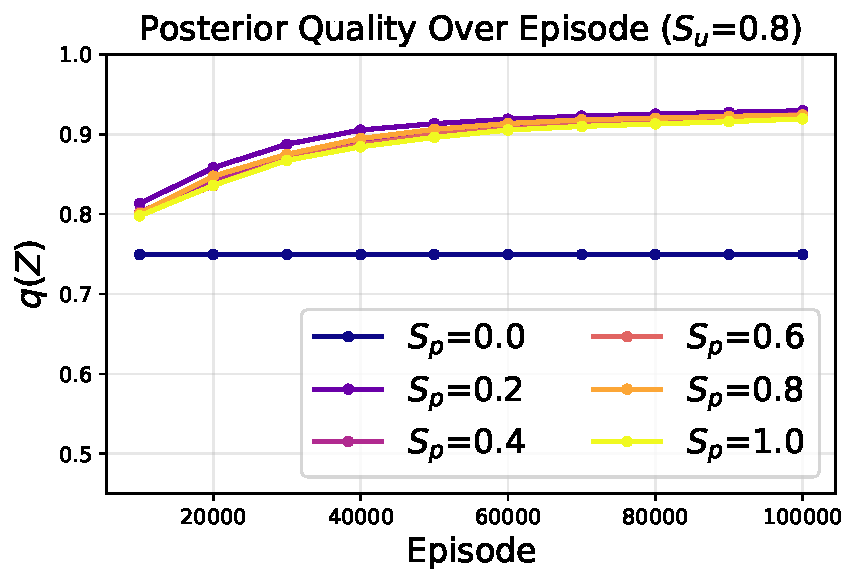
\includegraphics[width=\linewidth]{figures/fixed_su/user_strategy_0_8_weighted_p.png}
%         \caption{0.8}
%     \end{subfigure}
%     % \hfill
%     \begin{subfigure}[b]{0.162\linewidth}
%         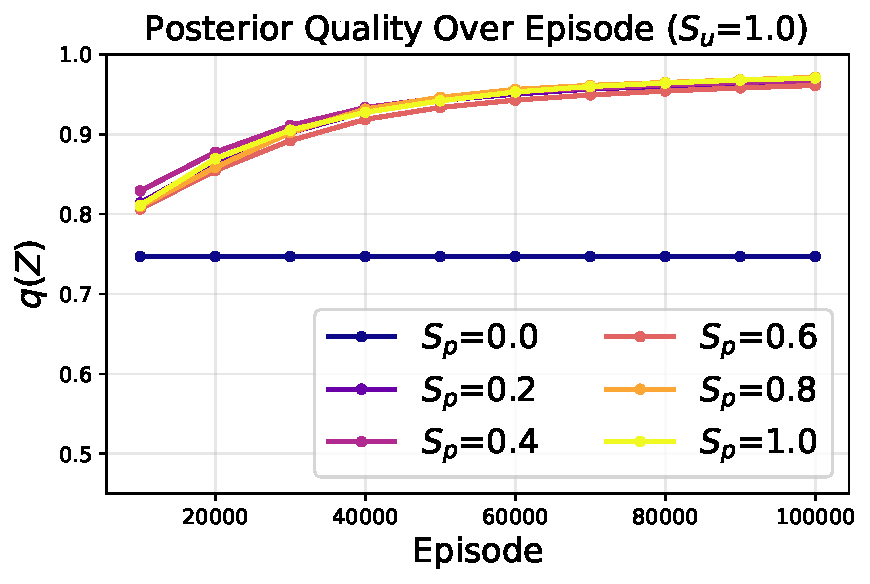
\includegraphics[width=\linewidth]{figures/fixed_su/user_strategy_1_0_weighted_p.png}
%         \caption{1.0}
%     \end{subfigure}
%     \caption{weighted p}
%     \label{fig:five-images}
% \end{figure*}



\begin{figure*}[t]
    \centering
    \vspace{-6mm}
    \begin{subfigure}[b]{0.195\linewidth}
        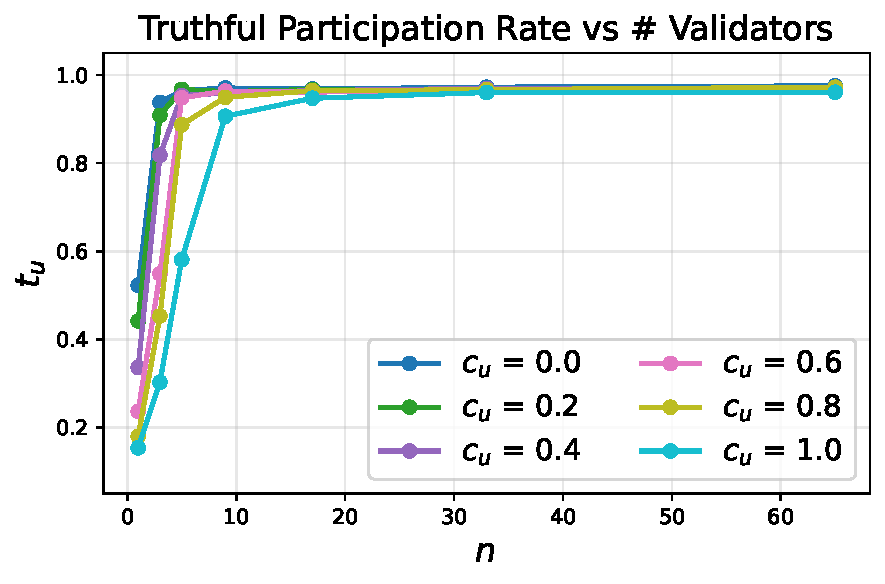
\includegraphics[width=\linewidth]{figures/hard/hard_all_costs.pdf}
        \caption{Truthful Participation}
    \end{subfigure}
    \hfill
    \begin{subfigure}[b]{0.195\linewidth}
        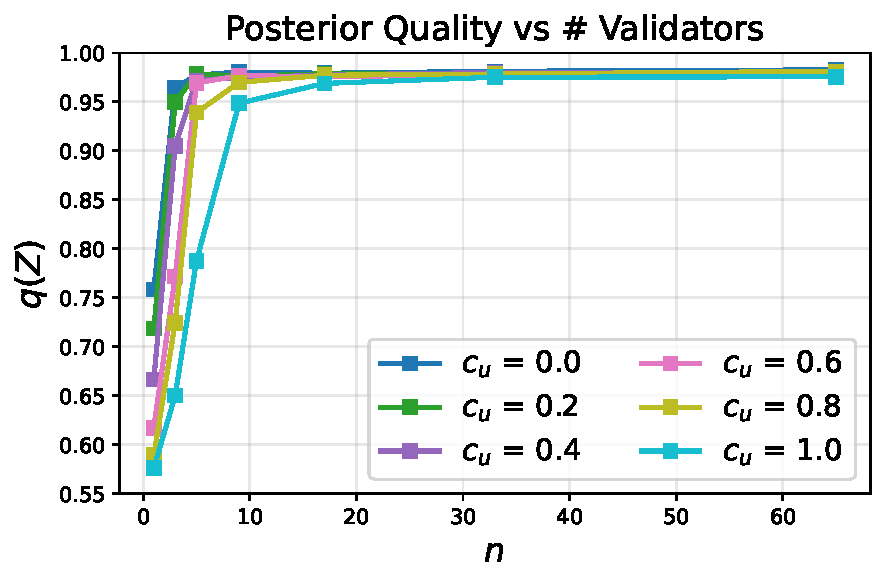
\includegraphics[width=\linewidth]{figures/hard/weighted_p_all_costs.pdf}
        \caption{Posterior Quality}
    \end{subfigure}
    \hfill
    \begin{subfigure}[b]{0.195\linewidth}
        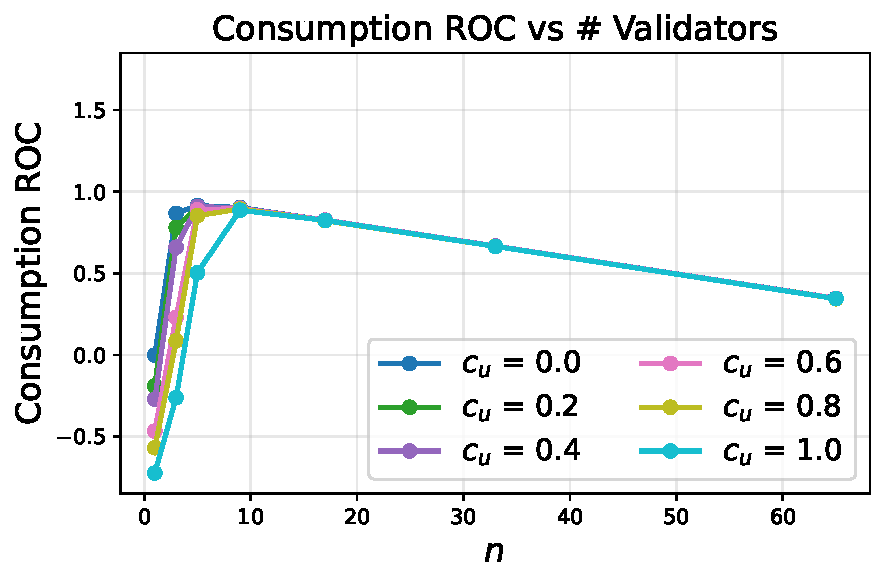
\includegraphics[width=\linewidth]{figures/hard/consumer_roc_all_costs.pdf}
        \caption{Consumption ROC}
    \end{subfigure}
    \hfill
    \begin{subfigure}[b]{0.195\linewidth}
        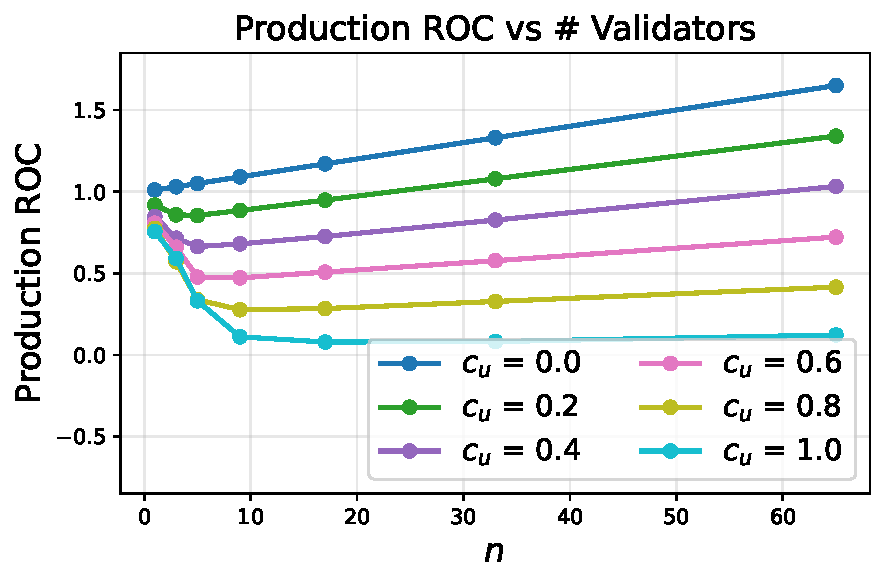
\includegraphics[width=\linewidth]{figures/hard/validator_roc_all_costs.pdf}
        \caption{Production ROC}
    \end{subfigure}
    \hfill
    \begin{subfigure}[b]{0.195\linewidth}
        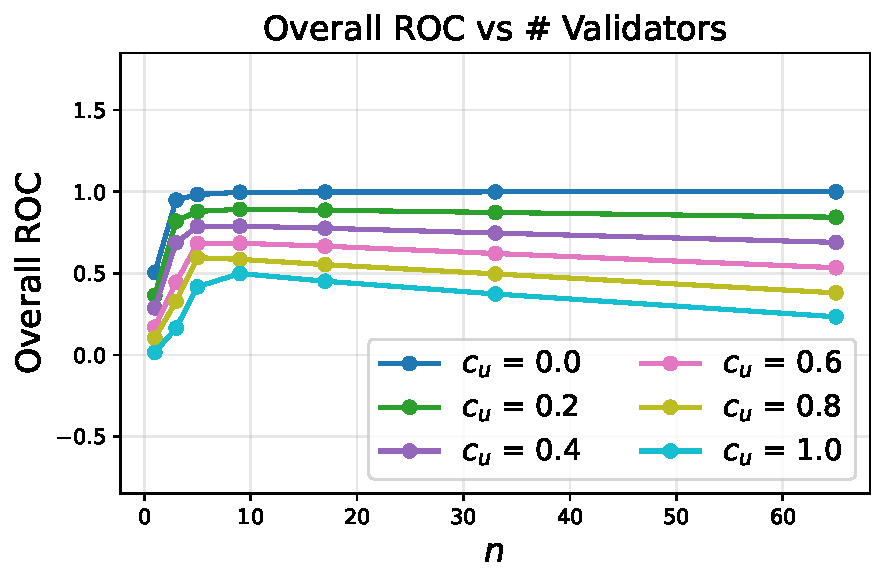
\includegraphics[width=\linewidth]{figures/hard/total_roc_all_costs.pdf}
        \caption{Overall ROC}
    \end{subfigure}
    \vspace{-2mm}
    \caption{Performance comparison with different cost and number of validators.}
    \label{Performance comparison with different cost and number of validators}
    \vspace{0mm}
\end{figure*}

\begin{figure*}[t]
    \centering
    \begin{subfigure}[b]{0.15\linewidth}
        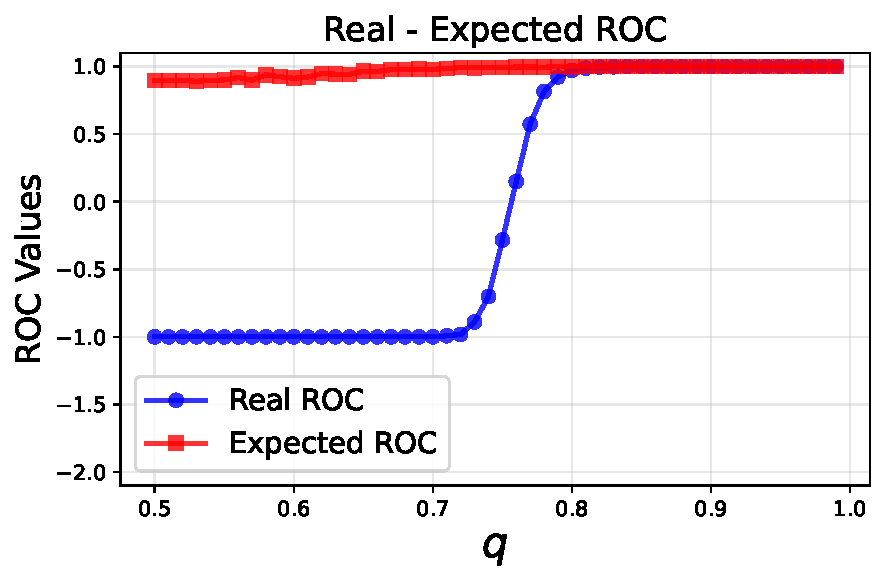
\includegraphics[width=\linewidth]{figures/quality/real_expected_roc_vs_p.pdf}
        \caption{Real ROC - \\Expected ROC}
    \end{subfigure}
    % \hfill
    \begin{subfigure}[b]{0.15\linewidth}
        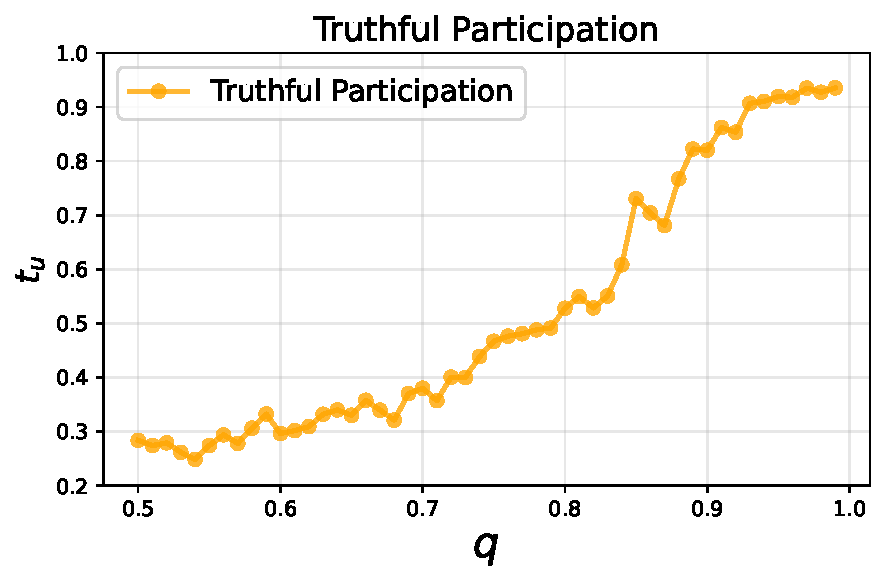
\includegraphics[width=\linewidth]{figures/quality/truthful_participation_vs_p.pdf}
        \caption{\textbf{\footnotesize Truthful \\Participation}}
    \end{subfigure}
    % \hfill
    \begin{subfigure}[b]{0.15\linewidth}
        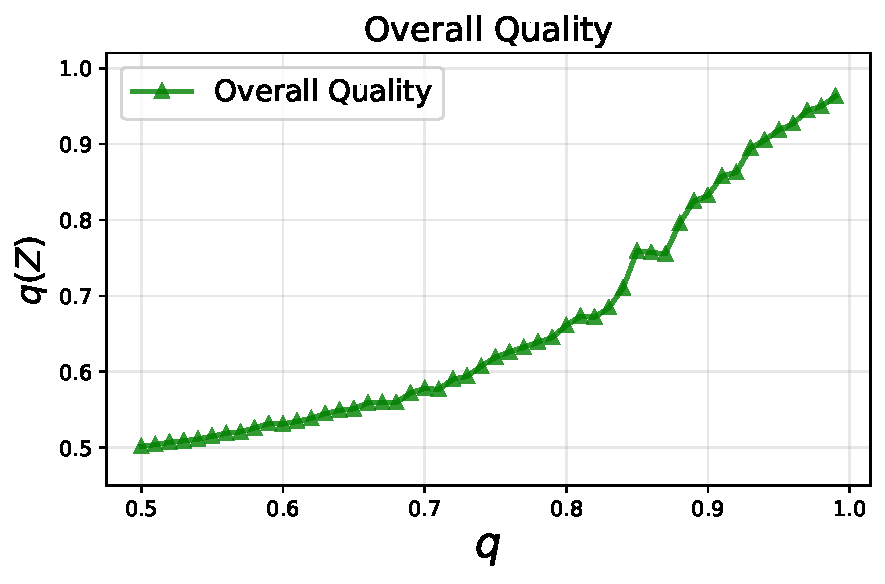
\includegraphics[width=\linewidth]{figures/quality/posterior_quality_vs_p.pdf}
        \caption{Overall \\Quality}
    \end{subfigure}
    % \hfill
    \begin{subfigure}[b]{0.15\linewidth}
        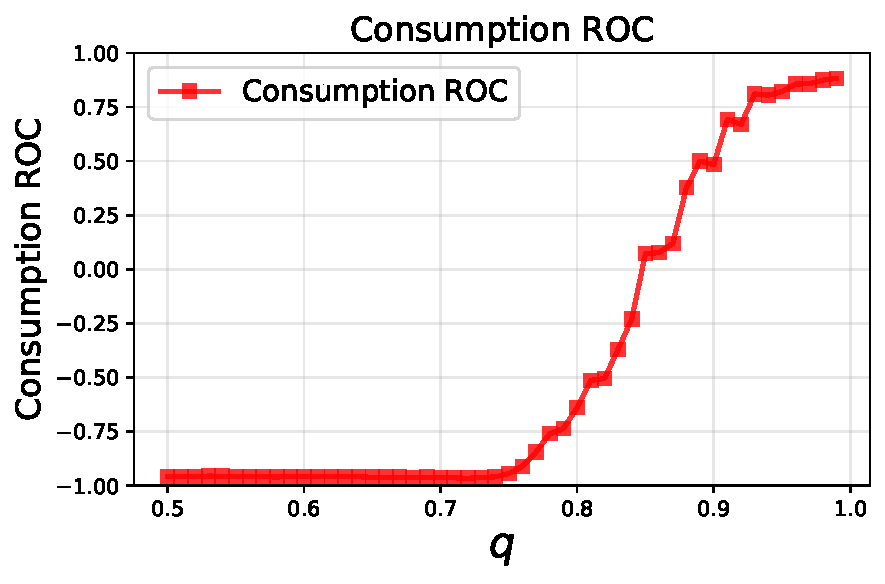
\includegraphics[width=\linewidth]{figures/quality/consumption_roc_vs_p.pdf}
        \caption{Consumption \\ROC}
    \end{subfigure}
    % \hfill
    \begin{subfigure}[b]{0.15\linewidth}
        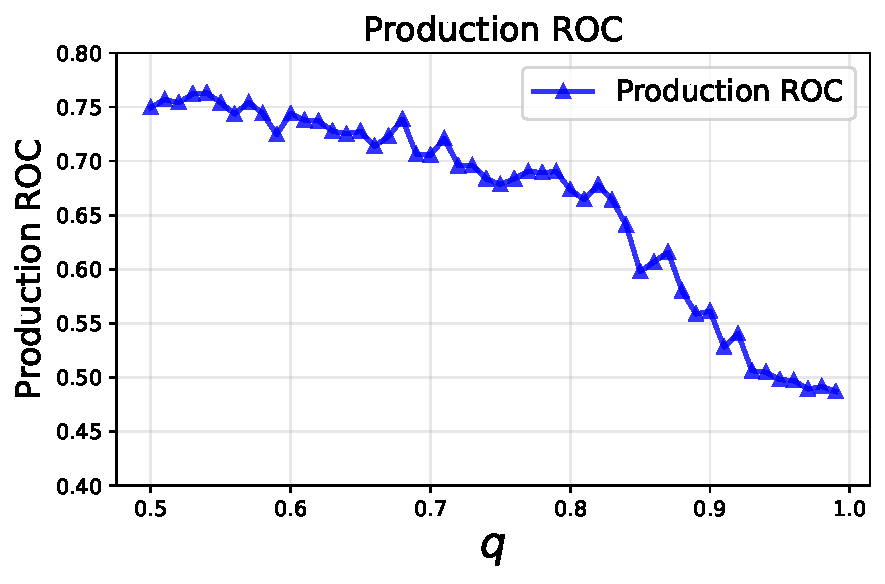
\includegraphics[width=\linewidth]{figures/quality/production_roc_vs_p.pdf}
        \caption{Production \\ROC}
    \end{subfigure}
    % \hfill
    \begin{subfigure}[b]{0.15\linewidth}
        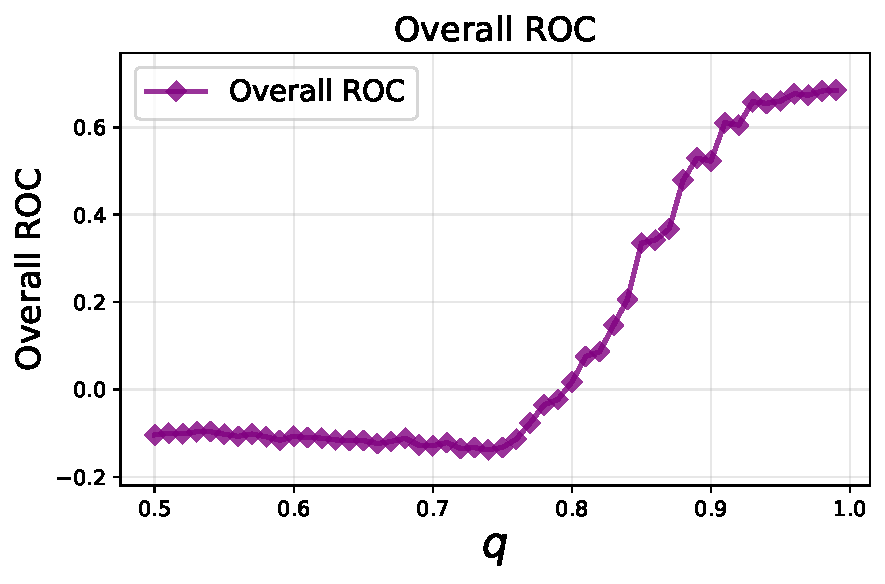
\includegraphics[width=\linewidth]{figures/quality/total_roc_vs_p.pdf}
        \caption{Overall \\ROC}
    \end{subfigure}
    \vspace{-2mm}
    \caption{Performance comparison with different service quality.}
    \label{erformance comparison with different service quality}
\end{figure*}

\vspace{-2mm}
\subsection{Simulation Setting}
We make the following assumptions. 
\textbf{(1) Users and Roles.}
The system contains $N=10000$ users, each randomly acting as a consumer, producer, or validator in each round.
Consumers raise information-seeking queries uniformly, while other users can respond or validate.
Assume the user service quality satisfies $q \sim 0.98 + 0.02\mathrm{Beta}(4,4) > \frac{1}{2}$, and when selected randomly, $q = \frac{1}{2}$. Each user starts with 2000 tokens and exits once depleted.
\textbf{(2) Validation Mechanism.}
Validator number $n$ is odd and chosen from $\{1,5,9,17,33,65\}$ and each validation uses $m=10$ samples.
Evaluation fee $\tau_{\text{val}}=1$, stake $\sigma=1$, and consensus is reached by majority vote. We define a basic strategy as adjusting their truthful participation rate in both production and validation.
Assuming users aim to maximize their return on capital (ROC), low-ROC users tend to learn strategies from high-ROC users. The initial strategy is random, i.e. $t_u =\text{Uniform}(0,1)$.
\textbf{(3) Promotion and Subscription.}
Producers incur effort cost $c_u\in(0,1)$ for one query validation and receive $\tau_s=1000$ upon subscription. 
\textbf{(4) System Assumptions.}
Validators are independent and non-collusive. All parameters are finite constants or drawn from bounded intervals. We do not consider adversarial attacks such as Sybil attacks or validator collusion.
We simulate 100,000 interactions and evaluate the following metrics:
(1) truthful participation rate $t_u$.
(2) ROC, reflecting individual or community benefit; and
(3) posterior quality $q(Z)$.

\subsection{User Rationality and Community Evolution}

We discuss how user rationality influences the evolutionary dynamics of the community by examining the overall ROC.
Users are categorized into the production side and consumption side, depending on whether they provide or request services.
Their respective ROCs are analyzed separately to reveal structural differences between producers and consumers. At the population level, $S_p$ denotes the proportion of users adhering to potentially rational strategies, while $S_u$ represents the probability that these users actually adjust their strategies. As shown in Figure~\ref{ROC Comp}, when $S_u = 1$ but $S_p = 0$, that is, users never update their strategies, the producer surplus exceeds the consumer surplus, yet the overall welfare remains lower than in cases where users adapt their strategies.
When rational producers refine strategies according to $t_u$, their labor cost increases and their individual surplus decreases, but the improved service quality enhances consumer surplus and raises total social welfare. Similarly, in Figure~\ref{ROC Comp}, low-ROC users strive to increase their competitiveness by self-improving $t_u$, as shown in Figure \ref{Truthful participation comparison}.
This implies that rational producers are intrinsically motivated to optimize their strategies and make truthful contributions, which in turn encourages broader collective improvement.
Consequently, such an incentive-compatible economic mechanism drives producers toward honest and diligent behavior until social welfare is maximized.

\vspace{-2mm}
\subsection{Validation Mechanism Analysis}

We examine how the number of validators influences both their truthful participation and the corresponding posterior service quality, and further analyze the ROCs for the consumption side, production side, and the system as a whole. 
As shown in Figure \ref{Truthful participation comparison}(a), when the requester invites only one validator, the validator can directly manipulate the consensus result due to the lack of competition. 
In this case, the validator tends to be lazy, and the saved effort cost becomes their surplus, while consumers suffer losses from decisions made based on incorrect validation outcomes.
As more validators participate, producers develop mutual supervision and the validators exert effort to avoid being forfeited. 
Therefore, as shown in Figure \ref{Truthful participation comparison}(b), truthful validation becomes the dominant consideration, and the posterior quality of voting results improves significantly with increasing $n$. 
Although the validation cost rises with $n$, consumer benefits exhibit diminishing marginal returns, and $t_u$ decreases marginally, while the overall validation revenue grows with $n$. 
Consequently, as depicted in Figures \ref{Truthful participation comparison}(c) and \ref{Truthful participation comparison}(e), social welfare and consumer surplus first increase and then decline with $n$, whereas producer surplus in Figure \ref{Truthful participation comparison}(d) first decreases and later increases.

\vspace{-3mm}
\subsection{Service Quality Impacts}

To investigate the impact of service quality on social welfare, we compare multiple metrics under different quality levels. As shown in Figure \ref{erformance comparison with different service quality}(a), when producers’ service quality is generally low, the validation results observed by consumers deviate substantially from the truth. Consequently, consumers make subscription decisions based on incorrect signals and suffer welfare losses. In the extreme case of $q=0.5$, producers cannot obtain higher incentives through providing reliable services and thus become increasingly idle in Figure \ref{erformance comparison with different service quality}(b), leading to negative growth in both consumer surplus and overall social welfare, as illustrated in Figures \ref{erformance comparison with different service quality}(d)(e)(f).
As illustrated in Figure \ref{erformance comparison with different service quality}(c), with the increase of $q$, producers’ service quality gradually improves. Their effort begins to receive positive feedback from the mechanism, which stabilizes the incentive environment: producer surplus slightly decreases as effort cost rises, while consumer surplus and total social welfare turn positive and continue to grow. When producers provide higher-quality services, they are more willing to exert effort, social welfare increases accordingly, and the incentive mechanism exhibits a stronger positive regulatory effect, as shown in Figures \ref{erformance comparison with different service quality}(e)(f).
